%% Einleitung.tex
%% $Id: einleitung.tex 61 2012-05-03 13:58:03Z bless $
%%

\chapter{Einleitung}
\label{ch:Einleitung}
%% ==============================
Die Einleitung besteht aus der Motivation, der Problemstellung, der Zielsetzung und einem erster Überblick über den Aufbau der Arbeit.

%% ==============================
\section{Motivation}
%% ==============================
\label{ch:Einleitung:sec:Motivation}
Das \emph{Knotenüberdeckungsproblem}, oder englisch Vertex Cover, ist ein nachgewiesen NP-vollständiges Problem \cite{intract}. Um das Problem zu erklären, betrachten wir ein Netz von Haushalten, bei dem wir die Möglichkeit haben, in jedem Haushalt einen Stromgenerator zu platzieren, sodass durch alle mit diesem Haus verbundenen Leitungen Strom fließt. Ziel ist, ein stabiles Stromnetz zu schaffen, bei dem jede Leitung an mindestens eine Stromquelle angeschlossen ist. Nun ergibt sich das Problem, dass die Kosten für Stromgeneratoren erheblich sind und daher nur maximal \emph{k} Geräte angeschafft werden können. Es gilt also, aus den \emph{n} Häusern \emph{k} oder weniger auszuwählen, sodass jede Leitung von einem der Häuser in der Auswahl versorgt wird. 
\begin{figure}[htb]
\centering
  	{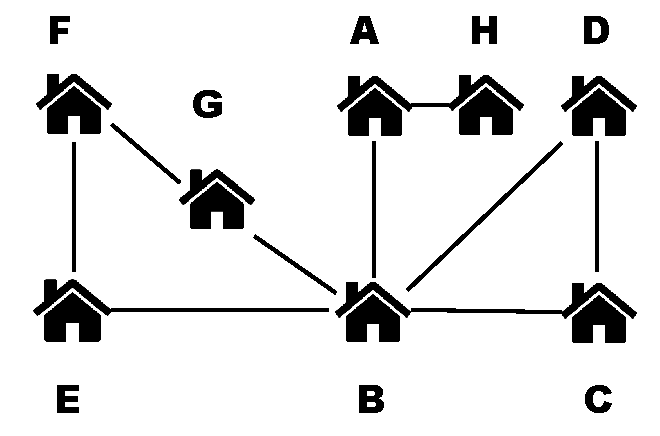
\includegraphics[width=.5\textwidth]{vertexcoverBsp.pdf}}
	\caption{Graph eines Stromnetzes \label{fig:vc}}
\centering
\end{figure}
In Abbildung \ref{fig:vc}\footnote{Icons in der Graphik von https://www.flaticon.com/}   sieht man ein Beispiel für eine solche Probleminstanz. Die Haushalte sind jeweils mit einem Buchstaben gekennzeichnet; jede Linie, beziehungsweise Kante eine Leitung zum Nachbarhaus. Hier ist es möglich eine Lösung für \emph{k} = 4 zu finden, also 4 Häuser mit Generatoren auszustatten, sodass alle Leitungen versorgt sind. Es ist leicht zu sehen, dass es keine Lösung mit weniger Häusern gibt. Um 4 Häuser, die das Problem lösen zu finden, betrachtet man nun jede Leitung und entscheidet, welches der beiden Häuser aufgenommen werden soll, da mindestens eins der beiden Häuser in der Lösungsmenge ist. Werden alle $2^{8}$ Möglichkeiten ausprobiert, finden sich die Lösung, dass wenn die Haushalte F, B, A und C oder F, B, A und D mit einem Generator ausgestattet werden, durch alle Leitungen Strom fließt. Für eine Problemgröße wie sie hier geschildert wird, bietet die \emph{Brute-Force}-Methode eine Lösung. Für eine Häusermenge \emph{n} = 2000 mit entsprechend vielen Leitungen bedeutet das ungefähr $1.148 \cdot 10^{602}$ mögliche Kombinationen. Die akzeptierten Kombinationsmöglichkeiten werden zwar durch \emph{k} begrenzt, was allerdings immernoch $2000 \choose k$ Proben bedeutet.


Es ist leicht zu sehen, dass sich das Stromnetzproblem, ersetzt man die Häuser durch Knoten eines Graphen und die Leitungen durch dessen Kanten,  zum Knotenüberdeckungsproblem transformieren lässt, welches sich folgendermaßen definiert\cite{trees}:
\begin{align*}
EINGABE: &\ Graph\ G=(V,E),\ positive\ Integer\ k\leq |V|\\
AUSGABE: &\ S\subseteq V\ mit\ |S|\leq k,\\
&\ sodass\ jede\ Kante\ aus\ E\ einen\ Endpunkt\ in\ S\ hat.
\end{align*}
Ein nichtdeterministischer Algorithmus kann jede vermeintliche Lösungskombination aus Knoten, beziehzungsweise Haushalten in Polynomialzeit testen \cite{intract}, da lediglich überprüft werden muss, ob die Größe der Lösungsmenge den Wert von \emph{k} überschreitet und ob alle Kanten abgedeckt (Leitungen versorgt) sind.
 Allerdings würde ein naiver Algrithmus für große Eingaben in der Realität nicht in absehbarer Zeit terminieren, wie beispielhaft in Tabelle \ref{tab:exponential} zu sehen ist.
 
 \begin{table}[htb]
\caption{Exponentielle Laufzeit \label{tab:exponential}}
\vspace*{1em}
\centering

\bgroup
\def\arraystretch{1.3}%  1 is the default, change whatever you need

\begin{threeparttable}

\begin{tabular}[c]{ l | l }
	
	\multicolumn{1}{c|}{\textbf{Eingabegröße}} & 
	\multicolumn{1}{c}{\textbf{Laufzeit}} \\ 
	
	\hline

	$2^{1}$& 0.00002s\\
	$2^{10}$& 0.02s\\
	$2^{100}$& ca. $ 2 \cdot 10^{14} $ Jahrtausende \\
	
\end{tabular}

\begin{tablenotes}\footnotesize
\item EINFÜGEN
\end{tablenotes}

\end{threeparttable}

\egroup

\end{table}
Es scheint also sinnvoll zu sein, die Eingabe möglichst klein zu halten und zu \emph{reduzieren}, indem einfache Teile des Graphen durch Vorverarbeitung (englisch \emph{Preprocessing}) entfernt werden und gegebenenfalls in die Lösungsmenge aufgenommen werden. Hierfür bieten sich einige einfache Beobachtungen, die über einen Graphen getroffen werden können an. Auf das Stromnetzproblem mit einem Netz mit maximal \emph{k} Generatoren bezogen bedeuten diese: 
\begin{enumerate}
\item Häuser, die isoliert stehen und keine Leitungen haben, können aus dem Netz entfernt werden
\item Bei Häusern, die genau eine Leitung, beziehungsweise genau ein Nachbarhaus haben, bekommt entsprechende Nachbarhaus automatisch einen Stromgenerator (Grad$_{1}$-Regel)
\item Häuser, die $k+1$ Leitungen zu anderen Häusern haben, erhalten einen Generator, da sonst alle Nachbarnhäuser versorgt würden und somit mehr Generatoren, als verfügbar verteilt werden müssten (Buss-Regel)
\end{enumerate}
Angewandt an eine Probleminstanz bedeutet das Einsetzen einer der Regeln, dass die entsprechenden Häuser und Leitungen von einer weiterführenden Betrachtung ausgeschlossen sind. Es entsteht ein äquivalenter, kleinerer Problemkern. Dies geschieht durch die meißten Regeln in polinomieller Zeit, um dann im Nachhinein einen langsameren Algorithmus für das Lösen des Problems zu benutzen \cite{param}. Das Beispiel in Abbildung \ref{fig:vc} kann durch die wiederholte Anwendung der Regeln sogar gelöst werden:
\begin{enumerate}
\item Es stehen 4 Generatoren zur Verfügung, allerdings hat Haus B 5 ausgehende Leitungen $\Rightarrow$ Buss-Regel: B erhält einen Generator und dessen Leitungen haben Strom.
\item Drei disjunkte Mengen von Häusern (\{E, G, F\}, \{D, C\} und \{A, H\}) bleiben übrig, wo jeweils einmal die Grad$_{1}$-Regel angewandt werden kann. Die 3 restlichen Generatoren werden verteilt, wobei sich bei jeder der Häusergruppen mehrere Möglichkeiten bieten.
\item Es steht kein Generator mehr zur Verfügung und aus der Restmenge {E, G, F} bleibt ein Haus ohne stromlose Leitungen zurück $\Rightarrow$ das Haus wird aus der Betrachtung entfernt und das Problem ist gelöst.
\end{enumerate}
Nach der wiederholten Anwendung der Buss-Regel haben alle Häuser mit mehr als \emph{k} Leitungen einen Generator und sind von der weiteren Betrachtung ausgeschlossen. Jeder übrige Haushalt kann also maximal \emph{k} stromlose Leitungen haben. Wenn nun noch mehr als $k^{2}$ Leitungen zu versorgen sind, kann es keine Lösung dieser Probleminstanz geben, da lediglich \emph{k} Stromgeneratoren zur Verfügung stehen und, verteilt auf die Häuser, somit nur maximal $k^{2}$ Leitungen unter Strom setzen können. Es bleiben höchstens $2 k^{2}$ Häuser ohne Generator (mit mindestens einer Leitung), bei denen noch nicht alle Leitungen Strom haben übrig\cite{param}, da jede der Leitungen an 2 Häusern angeschlossen ist. Wird nun die Grad$_{1}$-Regel angewandt bis sie nicht mehr greift, sind höchstens $k^{2} + k$ Häuser übrig, da jedes dieser Häuser jetzt zwischen 2 und \emph{k} stromlose Leitungen hat.


Um ein Haus unter den \emph{n} Häusern mit mehr als \emph{k} Leitungen zu finden, werden im schlimmsten Fall $k \cdot n$ Schritte benötigt, da für jedes Haus alle Leitungen gezählt werden müssen. Falls alle Häuser \emph{k} Leitungen haben, wird die Buss-Regel nicht ausgelöst. Ansonsten wird das gefundene Haus mit all seinen Leitungen aus dem Netz entfernt, was wiederum $p = k + x\ (\text{mit}\ x \geq 1)$ Schritte benötigt, wobei \emph{p} die Anzahl an Leitungen ist. Die Grad$_{1}$-Regel benötigt im schlimmsten Fall $2 \cdot n$ Schritte um das Häusernetz einmal zu durchlaufen, da die Betrachtung eines Hauses abgebrochen werden kann, sobald es mehr als eine Leitung hat, das es dann für diese Regel uninteressant ist. Wird ein Haus gefunden, kann dessen Nachbar und alle von diesem ausgehenden Leitungen entfernt werden, also $p$. Wird die Buss-Regel wurde vor der Grad$_{1}$-Regel angewandt, bedeutet das, dass maximal \emph{k} Schritte gebraucht werden. Um alle Häuser ohne Leitungen zu entfernen, muss lediglich für jedes Haus überprüft werden, ob es Leitungen hat, also \emph{n} Schritte.




In \emph{O}-Notation ergibt sich daraus eine Laufzeitabschätzung eines Durchlaufs von
\begin{align}
\text{Worst Case}:\ & kn + p + p + 1\\
\Rightarrow\ & O(kn + p)\\
\Rightarrow\ & O(kn)
\end{align}

Um größere Instanzen weiter zu vereinfachen stehen allerdings auch weiteaus komplexere Reduktionsregeln zur Verfügung. In dieser Arbeit werden das Nemhauser-Trotter-Theorem, beziehungsweise die dazugehörige Reduktionsregel und die Kronenregel betrachet.


Eine schnelle Laufzeit, um eine Knotenüberdeckung in einem gegebenen Graphen \emph{G}, Parameter \emph{k} und einer Knontenmenge \emph{n} zu finden wird von Chen et al \cite{paper:4} mit $O(kn + 1.271^{k}k^{2})$ vorgeschlagen; die schnellste bekannte Methode, alle Knotenüberdeckungen eines Graphen zu zählen von Mölle et al \cite{paper:5} mit einer Laufzeit von $O(1.3803^{k})$.

%% ==============================
\section{Problemstellung}
%% ==============================
\label{ch:Einleitung:sec:Problemstellung}

Reihenfolge der Reduktionen (Beispiel beachten). Der Graph wird dauerhaft verändert.

\begin{itemize}
\item Effekt von Graphreduktionsalgorithmen auf die Problemkomplexität
\end{itemize}

%% ==============================
\section{Zielsetzung}
%% ==============================
\label{ch:Einleitung:sec:Zielsetzung}

\begin{itemize}
\item Kategorisierung der Regeln?
\item Bewertungskriterien für einen GRalgorithmus
	\begin{itemize}
	\item Laufzeit (Parametrisierung)
	\item Erwartete Reduktion/Wie oft wird die Regel angewandt
	\item Ressourcenverbrauch
	\item Wie gut ist das Ergebnis im Vergleich zu anderen Algorithmen?	
	\end{itemize}
\item Wie funktionieren die GRA in Kombination?
\item Wie sehen Graphen aus, auf die keine Regel anwendbar ist?
\item Wie sehen Graphen aus, auf die genau eine Regel anwendbar ist?
\item Welche Regeln werden untersucht?
\end{itemize}


%% ==============================
\section{Gliederung/Aufbau der Arbeit}
%% ==============================
\label{ch:Einleitung:sec:Gliederung}

Was enthalten die weiteren Kapitel? Wie ist die Arbeit aufgebaut? Welche Methodik wird verfolgt?


%%% Local Variables: 
%%% mode: latex
%%% TeX-master: "thesis"
%%% End: 
